\documentclass[12pt, a4paper, oneside]{ctexbook}
\usepackage[margin=2cm]{geometry}%要先设置页边距,否则页眉页脚会偏
\usepackage{amsmath, amsthm, amssymb, bm, graphicx, hyperref, mathrsfs,float,xcolor,color}
\usepackage{listings}
\usepackage{ctex}

% 用来设置附录中代码的样式

\lstset{
    basicstyle          =   \bf \ttfamily,          % 基本代码风格
    keywordstyle        =   \bfseries,   % 关键字风格
    keywordstyle        =   \color{blue},
    stringstyle         =   \color{magenta},
    commentstyle        =   \color{red}\ttfamily,
    language            =    [x86masm]Assembler,
    commentstyle        =   \rmfamily\itshape,  % 注释的风格,斜体
    stringstyle         =   \ttfamily,  % 字符串风格
    flexiblecolumns,                % 别问为什么,加上这个
    numbers             =   left,   % 行号的位置在左边
    showspaces          =   false,  % 是否显示空格,显示了有点乱,所以不现实了
    numberstyle         =   \zihao{-5}\ttfamily,    % 行号的样式,小五号,tt等宽字体
    showstringspaces    =   false,
    captionpos          =   t,      % 这段代码的名字所呈现的位置,t指的是top上面
    frame               =   lrtb,   % 显示边框
}
\title{{\Huge{\textbf{微机系统与接口}}}}
\author{Leo}
\date{\today}
\linespread{1.2}
\newtheorem{theorem}{定理}[section]
\newtheorem{definition}[theorem]{定义}
\newtheorem{lemma}[theorem]{引理}
\newtheorem{corollary}[theorem]{推论}
\newtheorem{example}[theorem]{例}
\newtheorem{proposition}[theorem]{命题}

\begin{document}

\newcommand{\noindentbf}[1]{\noindent \textbf{#1} \quad}
\newcommand{\noindentbfline}[1]{\noindent \textbf{#1} \newline}

\maketitle

\newpage
\pagenumbering{Roman}
\setcounter{page}{1}
\tableofcontents
\newpage
\setcounter{page}{1}
\pagenumbering{arabic}

% 正文开始,chapter和section都放在子文件里
\chapter{8086CPU}
\section{计算机系统组成}
\subsection{计算机组成}
冯诺依曼结构的计算机分为外设和主机。外设就是输入输出设备,主机就是CPU(包括运算器和控制器)以及存储器
\subsubsection{工作原理}
\begin{enumerate}
    \item 从输出设备将数据或指令送到运算器
    \item 运算结果送给存储器或输出设备
    \item 从存储器取出数据到运算器再运算
    \item 从存储器取出指令送给控制器,译码分析后产生各种命令(上述动作都是由指令产生的各种命令控制的)
\end{enumerate}
\begin{figure}[H]
    \centering
    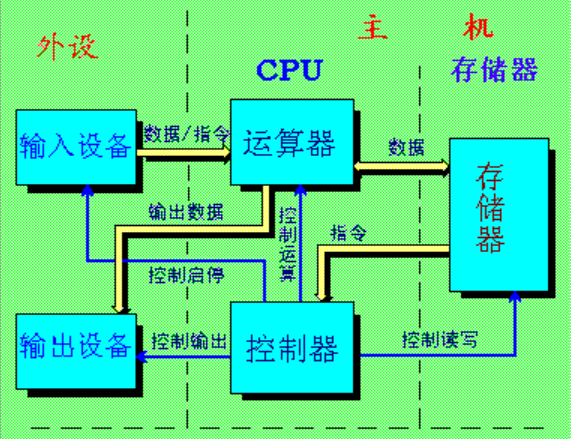
\includegraphics[scale=1]{part_8086CPU/part_8086CPU_pic/冯诺依曼计算机体系结构.png}
    \caption{冯诺依曼计算机体系结构图}
\end{figure}
\subsection{微机组成}
\begin{figure}[H]
    \centering
    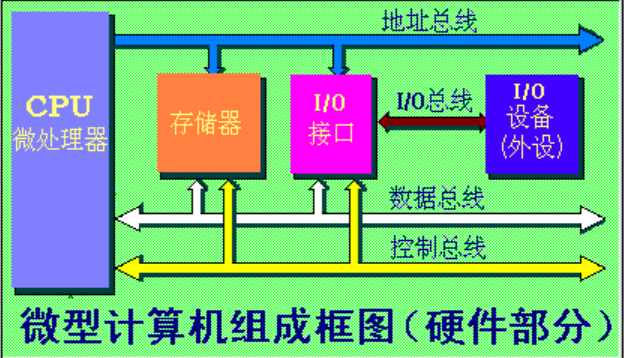
\includegraphics[scale=1]{part_8086CPU/part_8086CPU_pic/微机组成框图.png}
    \caption{微机组成框图}
\end{figure}
微型计算机由CPU微处理器、存储器、IO接口和IO设备(外设)组成
有4种总线
\begin{enumerate}
    \item 地址总线:连接CPU和存储器与IO接口
    \item 数据总线:连接CPU和存储器与IO接口
    \item 控制总线:连接CPU和存储器与IO接口
    \item IO总线:连接IO接口和IO设备
\end{enumerate}
工作过程
\begin{enumerate}
    \item 输入设备把指令送入IO接口,经过数据总线送入指定存储单元,存储器的地址由地址总线给出
    \item CPU从存储器取指令,产生地址、数据、控制信号,分别可以选中存储单元或端口、与选中的单元或接口交换数据、控制其他信号
\end{enumerate}
下面细讲各组成部分
\subsubsection{CPU}
即中央处理单元,计算机所有操作均在CPU的控制下进行,CPU型号直接决定了计算机的档次

Intel:
\begin{enumerate}
    \item 4004:4位微机
    \item 8085/8080:8位
    \item 8086/8088:16/准16位PC/XT机
    \item 80286:16位PC/XT机
    \item 80386/80486:32位机
    \item Pentium:奔腾32/64位机
\end{enumerate}
Motorola:6800(8位)——68000(16位)

Zilog:Z80(8位)——Z8000(16位)
\subsubsection{总线:BUS}
按传送的信息类型可以分为3类
\begin{enumerate}
    \item 数据总线:双向传送数据信息。可以连接多个设备,但是同一时间只能有一个设备在总线上(通过三态门控制)N根数据线可以同时传送N位信息。8086有16根,8088内部16,外部8根
    \item 地址总线:单向,用来寻址内存单元或IO端口。8086/8088都是20根
    \item 控制总线:输入输出,传送控制信号
\end{enumerate}
按规模、用途和应用场合可以分为3类
\begin{enumerate}
    \item 片级总线或元件级总线:用于芯片一级的互联,如CPU和存储器,CPU和IO接口
    \item 外部总线:也称为通信总线,用于微机和其他电子设备之间的连线
    \item 系统总线:也成为内总线和板级总线,用于微机中各插线板之间的连线
\end{enumerate}
\subsubsection{存储器:Memory}
用来存放数据和程序,每个存储单元存放一个字节,即8位bit。对每个存储单元编一个号,称为地址,地址单元和内容常常用16进制表示存储器中包含的字节数称为存储容量
\begin{figure}[H]
    \centering
    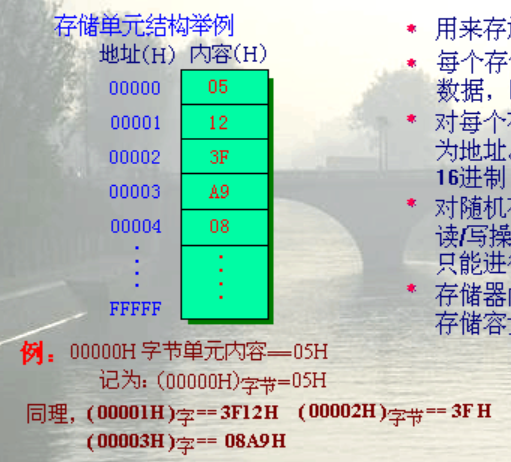
\includegraphics[scale=1]{part_8086CPU/part_8086CPU_pic/存储器结构举例.png}
    \caption{存储器结构举例}
\end{figure}
8086有20根地址线,可以直接寻址$2^{20}=1M$内存单元。使用了段加偏移的方法,一个物理地址有20位,可以表示为“段地址:偏移地址”=段地址*16+偏移地址

\noindentbfline{8086存储器}
一个程序可以有4个段,段名和段寄存器对应为
\begin{enumerate}\label{段寄存器4种}
    \item 代码段CS:code segment 将要执行的下一条指令一定是从CS:IP指示的单元中取出
    \item 数据段DS:data segment
    \item 堆栈段SS:stack segment
    \item 附加段ES:extra segment
\end{enumerate}
\subsubsection{IO接口}
为什么要有接口?因为外设与CPU交换数据的时候会带来一些问题
\begin{enumerate}
    \item 速度不匹配,一般是CPU远快于外设
    \item 信号电平不匹配
    \item 信号格式不匹配
    \item 时序不匹配
    \item 译码问题
\end{enumerate}
接口电路主要实现的功能
\begin{enumerate}
    \item 数据缓冲,使速度匹配:8255A通用并行接口、锁存器
    \item 电平转换:MC1488,MC1489,MAX233电平转换电路
    \item 串并行转换:8251A,8250串行接口芯片
    \item 数模模数转换:DAC0832,ADC0809
    \item 地址译码:74LS138
    \item 中断控制:8259A中断控制器
    \item 存储器直接数据传送控制:8237ADMA控制器
    \item 定时计数功能:8253,8254计数器/定时器
\end{enumerate}
\subsubsection{外设(即IO设备)}
输入设备:键盘、鼠标器、扫描仪、CD-ROM驱动器;

输出设备:CRT显示器、LPT打印机、扬声器、LED/LCD显示器
\subsection{微机系统组成}
\begin{equation}
    \begin{cases}
        \text{硬件}
        \begin{cases}
            \text{主机}
            \begin{cases}
                CPU\\
                \text{存储器}
            \end{cases}
            \text{各类接口芯片}\\
            \text{外设}
            \begin{cases}
                \text{输入设备}\\
                \text{输出设备}
            \end{cases}
        \end{cases}\\
        \text{软件}
        \begin{cases}
            \text{系统软件}
            \begin{cases}
                \text{操作系统:DOS、WINDOWS、UNIX}\\
                \text{汇编程序}\\
                \text{解释程序(对BASIC)}\\
                \text{编译程序(对高级语言)}
            \end{cases}\\
            \text{程序设计语言}
            \begin{cases}
                \text{机器语言}(\text{二进制码,计算机只认得这种语言})\\
                \text{汇编语言(符号语言)}\\
                \text{高级语言(C、FORTRAN、PASCAL)}
            \end{cases}\\
            \text{应用软件}
            \begin{cases}
                \text{软件包}\\
                \text{数据库}\\
                \text{文字处理软件、娱乐、教育等}
            \end{cases}
        \end{cases}
    \end{cases}
\end{equation}
\section{8086CPU系统}
\subsection{内部结构}
8086是16位,8088是准16位微处理器,都具有16位地址总线,可处理8或16位数据;外部都具有20根地址总线,可以直接寻址$2^{20}=1M$字节的内存空间,可以寻址$2^{16}=64K$个IO端口。

采用+5V供电,单相时钟

8086外部有16根地址总线,8088有8根,与外部传送数据时,都要执行外部总线周期。
\subsubsection{8086结构与原理}
\begin{figure}[H]
    \centering
    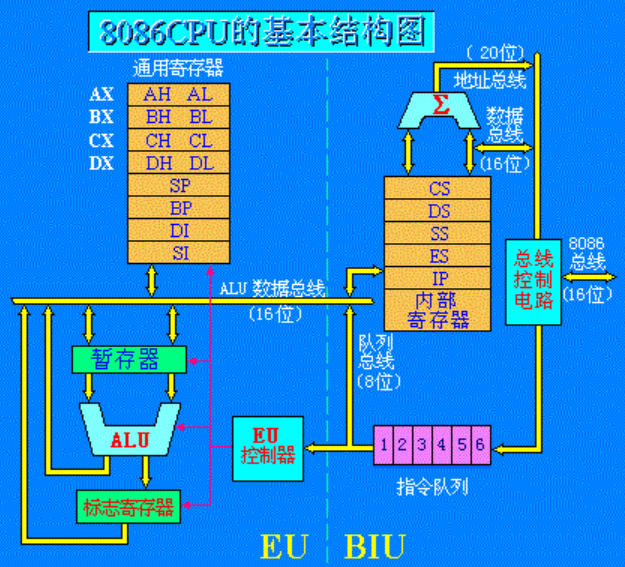
\includegraphics[scale=1]{part_8086CPU/part_8086CPU_pic/8086CPU基本结构.png}
    \caption{8086CPU基本结构}
\end{figure}
主要由两部分组成:

EU执行单元
\begin{enumerate}
    \item 负责执行全部指令
    \item 给BIU提供数据和地址信息
    \item 管理通用寄存器和标志寄存器,不直接和外部打交道
\end{enumerate}
BIU总线接口单元
\begin{enumerate}
    \item 执行所有的外部总线周期
    \item 负责与存储器,IO端口打交道
\end{enumerate}
工作流程
\begin{enumerate}
    \item 读操作:BIU根据CS:IP在地址加法器形成20位物理地址,通过总线控制电路从mem中取出指令,送到6字节的指令队列中等待执行
    \item EU从队列中取指令,译码后执行。此时没有用到总线,BIU可继续工作,把队列填满。如果EU没有向BIU申请读或写存储器或IO操作时,BIU空闲(*在执行指令时预先取下一条指令的技术称为流水线)
    \item 若遇到JMP或CALL指令,队列中的内容作废,从新的转移地址中取指令码
    \item ALU完成算数/逻辑运算后,将运算结果通过数据总线送到EU的通用寄存器或暂存器;或者送到BIU的内部寄存器再送到存储器或IO端口。本次操作的状态反映在标志寄存器FLAGS中
\end{enumerate}
\subsubsection{8088内部结构}
与8086基本一样,主要区别在于:
\begin{enumerate}
    \item 8088指令队列为4字节,而不是6字节
    \item 8088外部数据总线为8位而不是16位
\end{enumerate}
\subsubsection{总线周期简述}
总线周期:在8086中,BIU完成一次访问存储器或IO端口的时间称为总线周期。最基本的总线周期由$T_1$到$T_4$4个时钟周期组成,也称为$T_1$到$T_4$状态。
\begin{figure}[H]
    \centering
    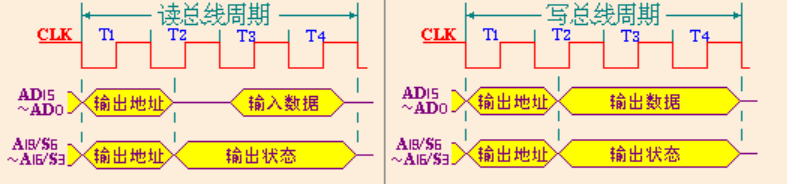
\includegraphics[scale=1]{part_8086CPU/part_8086CPU_pic/读周期和写周期.png}
    \caption{读周期和写周期}
\end{figure}
读周期:
\begin{enumerate}
    \item $T_1$状态通过4条地址/状态复用线和16条地址数据复用线(共20条线)向存储器输出指定地址
    \item $T_2$进入高阻态,缓冲一下,让AD地址数据复用线从输出地址变为输入数据信号。但是地址/状态复用线从$T_2$到$T_4$一直输出状态信号
    \item $T_3T_4$ 16条地址数据复用线接收指定单元内容
\end{enumerate}
\subsubsection{内部寄存器简述}
\begin{equation}
    \text{通用寄存器}
    \begin{cases}
        \text{数据寄存器}
        \begin{cases}
            \text{累加器AX}\\
            \text{基址寄存器BX}\\
            \text{计数寄存器CX}\\
            \text{数据寄存器DX}\\
        \end{cases}\\
        \text{指针和变址寄存器:涉及到存储器操作数时,可用的寄存器}
        \begin{cases}
            \text{堆栈指针SP:不能做通用寄存器}\\
            \text{基址指针BP}\\
            \text{源变址指针SI}\\
            \text{目的变址指针DI}
        \end{cases}
    \end{cases}\\
    \text{段寄存器}
    \begin{cases}
        \text{代码段指针CS}\\
        \text{数据段指针DS}\\
        \text{堆栈段指针SS}\\
        \text{附加段指针ES}
    \end{cases}\\
    \text{标志寄存器FLAGS}\\
    \text{指令指针IP}
\end{equation}
通用寄存器:16位寄存器用来存放数据和地址,8位的只能存放数据

数据寄存器隐含用途:
\begin{enumerate}
    \item AX:在字IO指令中,做16位数据寄存器;在字节乘法中存放乘积;在字节除法中存放被除数
    \item AH:字节除法中存放余数
    \item AL:字节IO指令中做8位数据寄存器;在字节乘法中存放乘数;在字节除法中存放商;BCD运算中必须将运算结果或被除数放在AL中才能用二-十进制调整指令调整;在XLAT指令中做指针和存放代码转换结果
    \item BX:做基地址指针;XLAT中存放表头地址
    \item CX:字符串操作和循环操作中做计数器
    \item CL:在算数逻辑移位和循环移位指令中做移位次数计数器
    \item DX:字乘法中存乘积的高半部分;字除法中存放被除数的高半部分和余数;在间接寻址的IO指令中做端口地址寄存器
\end{enumerate}
指针和变址寄存器隐含用途:
\begin{enumerate}
    \item SI:在字符串指令中做源串偏移地址指针
    \item DI:在字符串指令中做目的串偏移地址指针
    \item SP:在堆栈操作中指示栈顶位置
    \item BP:在堆栈操作中指示堆栈中一个数据区的偏移地址,可用于访问堆栈中的某个数据
\end{enumerate}
段寄存器:

计算机存储器中存放三类信息:代码信息,数据信息和堆栈信息,这三类信息存放在各自的内存区域中,用段寄存器来指示这些段的起始地址的高16位部分,一共有4种段寄存器\ref{段寄存器4种}

段寄存器和BX、BP、SI、DI等配合,可以构成多种寻址方式。例如CS:IP指出下一条要执行的指令的地址。SS:SP指向堆栈栈顶单元

标志寄存器:

16位FLAGS设置了9个标志位,其中6个为状态标志,用来反映上次运算结果的状态。另外三个为控制标志,用来控制CPU的某些操作
\begin{enumerate}
    \item OF(overflow)溢出标志:用于带符号数的运算,如果两个正数相加出现负数或者负数相加出现正数,则为1.(正确的结果也可能有进位,但是进位位自然丢失或给更高位)
    \item DF(direction)方向标志:控制SI、DI的变化方向。DF=0,则SI、DI自增;反之自减
    \item IF(interrupt)中断标志:STI指令使IF=1,允许CPU响应可屏蔽中断。CLI指令使IF=0,禁止CPU响应可屏蔽中断
    \item TF(trap)陷阱标志:TF=1,CPU处于单步工作方式,每执行一条指令自动内部中断,并打印信息,便于调试
    \item SF(sign)符号标志:数字的最高位MSB=1时,SF=1,表示结果为负值;MSB=0时,SF=0,表示结果为正值
    \item ZF(zero)零标志:运算结果为0时ZF=1
    \item AF(auxiliary)辅助进位标志:8位运算时,低半字节向高半字节有进位或借位时AF=1.16位运算时仅在低字节部分使用。一般用于BCD码运算的十进制调整(加6或减6)
    \item PF(parity)奇偶标志:算数逻辑运算时,结果有偶数个1时则PF=1,一般用来检验数据传输中的错误
    \item CF(carry)进位标志:最高位$D_7$或$D_{15}$产生进位或借位时CF=1
\end{enumerate}
指令指针

IP指针用来存放将要执行的下一条指令相对于现行代码段的偏移地址,用来控制指令序列的执行流程。

程序运行时,BIU自动对IP进行修改,使它始终指向下一条指令的地址。程序不能直接访问IP,只能由CPU自动控制
\subsection{存储器基础}
存储器主要用来存放程序和数据,存储容量和存取速度是决定性指标。内存容量一般指RAM大小
\subsubsection{存储器分类}
\begin{equation}
    \begin{cases}
        \text{内存}
        \begin{cases}
            RAM
            \begin{cases}
                SRAM\\
                DRAM
            \end{cases}\\
            ROM
            \begin{cases}
                ROM\\
                PROM\\
                EPROM\\
                E2PROM
            \end{cases}
        \end{cases}\\
        \text{外存}
        \begin{cases}
            \text{硬盘}\\
            \text{软盘}\\
            \text{磁带}\\
            \text{光盘}
        \end{cases}\\
        \text{高速缓冲存储器Cache}
    \end{cases}
\end{equation}
\subsubsection{8086分段概念}
为什么要分段?因为地址线有20根,但是CPU寄存器只有16位。

怎么分段?一个现行程序可以分为DS、CS、SS和ES四段,凡是能被16(或10H)整除的地址处均可分段。如00000H,00010H,00150H等

各段之间可以相互独立也可以相互覆盖

分段的好处?
\begin{enumerate}
    \item 大部分指令不涉及段寄存器的值,仅改变偏移量,这样可以缩短指令长度,提高运算速度
    \item 内存分段为程序的浮动装配创造条件
\end{enumerate}
\subsubsection{8086存储器结构}
8086可直接寻址的1MB内存分成2个512K的存储体,$A_0=0$选到偶地址体,$A_0=1$选到奇地址体。

CPU访问存储器都是从偶地址体开始的,以字为单位进行操作。读00000字时,从00000开始读两个字节,读出来的是(00001)(00000)代表的字;读00003字时,从00004开始读到00003,即读出内容为(00004)(00003)代表的字。

\noindentbfline{8086系统与存储器的连接}
\begin{enumerate}
    \item 每个存储器单元有8根数据线,奇地址体与CPU的高8位相连,偶地址体与低8位相连
    \item 用$A_0$和$\overline{BHE}$(Bus High Enable)来控制地址体的选中与否
\end{enumerate}
\begin{table}
    \centering
    \begin{tabular}[h]{c|c|c}
        \hline
        $\overline{BHE}$ & $A_0$ & 操作 \\ \hline
        0 & 0 &奇偶地址体都被选中,读字\\\hline
        0 & 1 &读偶地址体字节\\\hline
        1 & 0 &读奇地址体字节\\\hline
        1 & 1 &无操作 \\ \hline
    \end{tabular}
\end{table}
\subsubsection{8086堆栈操作}
一个堆栈不超过一个段的指示范围($2^{16}=64K$),由SS给出段基地址,SP存放偏移地址,指示栈顶位置,$SP\leq FFFEH$

堆栈的基本处理单元是字,压栈时,一个字的高8位先入栈,低8位后入栈,SP的值减二(注意16进制减法的不同)
\subsection{引脚功能}
\subsubsection{8086CPU引脚}
\noindentbf{$AD_{15}-AD_{0}$地址/数据总线}
分时复用:在总线周期的$T_1$状态,传送存储器或IO端口的地址信息,然后在ALE信号控制下用锁存器将$A_{15}-A_{0}$锁存住

$T_2$状态:读总线周期下为高阻态,写总线周期下,传送数据信号$D_{15}-D_0$

$T_3-T_4$状态:传送传送数据信号$D_{15}-D_0$

\noindentbf{INTR中断请求}
为高电平时,表示外部向CPU发送中断请求信号。CPU在每条指令的最后一个时钟周期都要对其信号进行采样,若为1,CPU的IF=1,则CPU转入中断响应周期

\noindentbf{NMI不可屏蔽中断}
CPU一旦检测到NMI的上跳变信号,则执行完当前指令后,进入类型2的不可屏蔽中断。这类中断不受IF影响,不能用软件屏蔽。

\noindentbf{CLK}
由外部时钟信号8284提供,基本在MHz级别

\noindentbf{$A_{19}S_{6}-A_{16}S_{3}$地址/状态总线}
分时复用:在总线周期的$T_1$状态做地址线用,可用于访问存储器,但是访问IO端口只用到低16位地址线,所以这四根线无效

$T_2-T_4$状态:输出状态信息
\begin{enumerate}
    \item $S_6=0$
    \item $S_5=1$允许可屏蔽的中断请求,$S_5=0$禁止可屏蔽的中断请求
    \item $S_4S_3$段寄存器状态线,从00到11分别表示当前正在使用的段寄存器为ES,SS,CS,DS
\end{enumerate}
\noindentbf{$\overline{BHE}/S_7$总线高位有效/状态线}
分时复用:$T_1$输出有效的$\overline{BHE}$信号。其他时候输出$S_7$,在8086中$S_7$无意义

\noindentbf{$MN/\overline{MX}$最小/最大模式} 

\noindentbf{$\overline{RD}$读信号}
执行读指令时该引脚变为低电平,到底是读存储器还是读IO取决于$M/\overline{IO}$信号

\noindentbf{READY准备好信号}由8284时钟信号产生器产生,一般CPU与低速外设交换数据时要等外设,此时READY变低电平,这样可以在$T_3$后插入若干等待周期$T_w$;READY变为高电平后,下一个周期进入$T_4$

\noindentbf{$\overline{TEST}$测试信号}CPU执行WAIT指令时,每隔5个T就检测一次该引脚,若为高电平(无效)则进入空闲周期,反之继续执行下一条指令

\noindentbf{RESET复位信号}高电平有效,至少维持4个时钟周期。复位时:
\begin{enumerate}
    \item CPU立即中止所有操作,总线无效
    \item IP,DS,ES,SS,FLAGS清零,CS=FFFFH,复位结束后,CS:IP=FFFF:0000H,CPU从这里开始执行程序,所以可在这里安排一条JMP RESET
    \item 指令队列清空
\end{enumerate}
\subsubsection{8088CPU引脚}
\noindentbf{$A_{15}-A_{8}$地址线}不与数据线复用,因为8088只需要8根数据线

\noindentbf{$SS_0$(High)}最小模式下为状态信号,与$IO/\overline{M}$,$DT/\overline{R}$一起决定现行总线周期的状态。最大模式下接高电平。

\noindentbf{$IO/\overline{M} (S_2)$}在8088中为1时访问IO,为0时访问存储器。在8086中反之
\subsection{工作模式}
$MN/\overline{MX}$接高电平时工作于最小模式:
\begin{enumerate}
    \item 系统中只有一个8086或8088微处理器
    \item 所有总线控制信号均由CPU直接产生或接收
\end{enumerate}
$MN/\overline{MX}$接低电平时工作于最大模式:
\begin{enumerate}
    \item 系统中允许多个处理器共同工作
    \item 有的控制信号由CPU直接产生,有的由8288总线控制器译码后产生
    \item 单个CPU也可以工作在最大模式
\end{enumerate}
两者的共同点:
\begin{enumerate}
    \item 都需要用地址锁存器8282/8283或74LS373(因为20位地址线,所以都要用三片芯片),使地址数据线先传送地址并锁存,再传送数据信号
    \item 都需要使用8286/8287或74LS245(8086用两片,8088用一片)控制数据传送的方向,同时增强数据总线的驱动力,在小系统中可以不用数据收发器。
\end{enumerate}
\subsubsection{8086最大模式}
\begin{figure}[H]
    \centering
    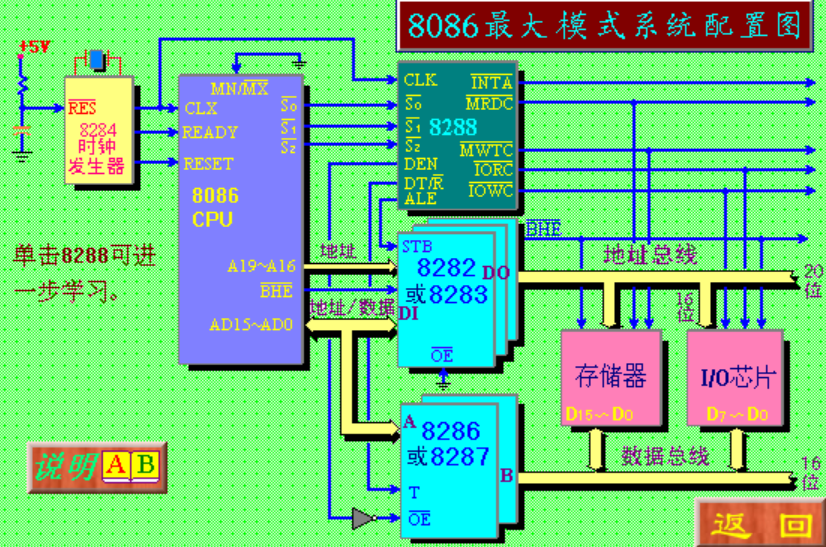
\includegraphics[scale=1]{part_8086CPU/part_8086CPU_pic/8086最大模式系统配置图.png}
    \caption{8086最大模式系统配置图}
\end{figure}
特征:
\begin{enumerate}
    \item $MN/\overline{MX}$接地
    \item 增加总线控制器8288来产生原来由CPU产生的控制信号
    \item 8288产生的ALE(地址锁存允许)、DEN(数据传送允许)和$DT/\overline{R}$(数据收发允许)三种信号与CPU一致
\end{enumerate}
\noindentbf{8288总线控制器}
接收时钟产生器送出的CLK信号,其频率与CPU的CLK相同。同时还接收CPU送来的状态信号,从输出端输出各种控制信号
\begin{enumerate}
    \item $DT/\overline{R}$,$ALE$:与最小模式信号相同
    \item DEN:与最小模式的$\overline{DEN}$相位相反
    \item $\overline{MRDC}$:存储器读,相当于$\overline{RD},M/\overline{IO}$结合,选中存储器。引到系统总线上命名为$\overline{MEMR}$
    \item $\overline{MWTC}$:存储器写,相当于$\overline{WR},M/\overline{IO}$结合,选中存储器。引到系统总线上命名为$\overline{MEMW}$
    \item $\overline{IORC}$:IO读,相当于$\overline{RD},M/\overline{IO}$结合,选中IO端口。引到系统总线上命名为$\overline{IOR}$
    \item $\overline{IOWC}$:IO写,相当于$\overline{WR},M/\overline{IO}$结合,选中IO端口。引到系统总线上命名为$\overline{IOW}$
    \item $\overline{INTA}$:中断响应信号
    \item *$\overline{AIOWC}$:超前写IO命令,与$\overline{IOWC}$相比,8288提前一个时钟周期向IO端口发出写命令。可以使较慢的设备提前一个周期进入写操作。用于PC机中。
    \item *$\overline{AMWC}$:超前写存储器命令,与$\overline{MWTC}$相比,8288提前一个时钟周期向存储器发出写命令
\end{enumerate}
\subsubsection{8086最小模式}
\begin{figure}[H]
    \centering
    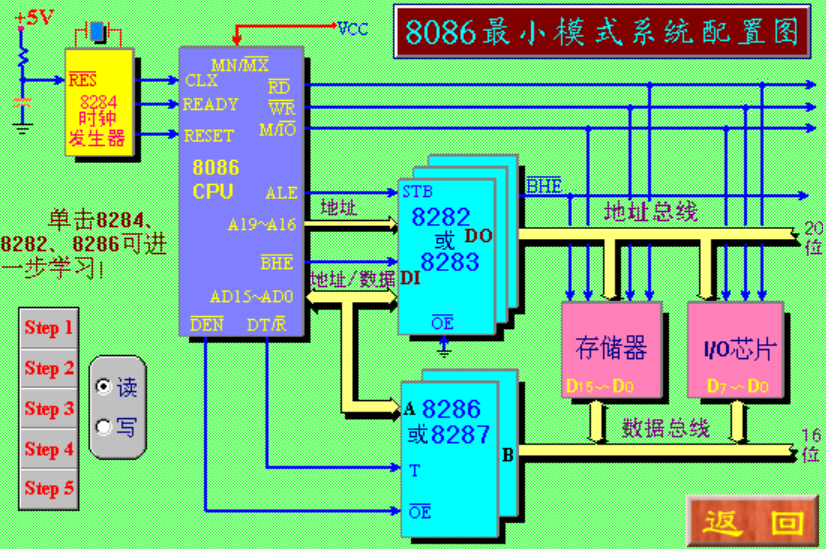
\includegraphics[scale=1]{part_8086CPU/part_8086CPU_pic/8086最小模式系统配置图.png}
    \caption{8086最小模式系统配置图}
\end{figure}
读存储器操作流程(读IO仅在第一步$M/\overline{IO}=0$处不一样)
\begin{enumerate}
    \item $M/\overline{IO}$置1选中存储器,$DT/\overline{R}$置零,使8286T引脚为零,使CPU准备接收数据
    \item 地址信号和$\overline{BHE}$输出给8282,同时送出一个ALE正脉冲,在ALE下降沿锁存
    \item 三态门打开,8282输出地址信号和$\overline{BHE}$到存储器某一指定单元
    \item CPU发出$\overline{RD}=0$读信号,同时CPU的$\overline{DEN}=0$使8286可以接收数据,且8286的T=0,允许接收数据
    \item 从选中的存储器单元中读出来送给8286,再送给CPU的$AD_{15}-AD_{0}$
\end{enumerate}

写存储器操作流程(写IO仅在第一步$M/\overline{IO}=0$处不一样)
\begin{enumerate}
    \item $M/\overline{IO}$置1选中存储器,$DT/\overline{R}$置1,使8286T引脚为1,使CPU准备发送数据
    \item 地址信号和$\overline{BHE}$输出给8282,同时送出一个ALE正脉冲,在ALE下降沿将20位地址和$\overline{BHE}$锁存
    \item 8282三态门打开,8282输出地址信号和$\overline{BHE}$到存储器某一指定单元
    \item CPU发出$\overline{WR}=0$读信号,同时CPU的$\overline{DEN}=0$使8286可以接收数据,且8286的T=1,允许发送数据
    \item CPU通过$AD_{15}-AD_{0}$把要写入的数据送给8286,再送到存储单元
\end{enumerate}
\noindentbf{8282地址锁存器(或用74LS373)}
\begin{figure}[H]
    \centering
    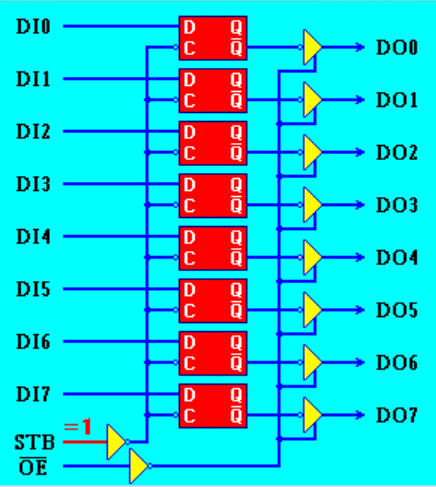
\includegraphics[scale=1]{part_8086CPU/part_8086CPU_pic/8282地址锁存器.png}
    \caption{8282地址锁存器}
\end{figure}
由8个D触发器和8个三态门组成,有STB和$\overline{OE}$两个控制端。STB=1时D触发器透明,STB产生下降沿时,锁存,STB=0时D端变化Q不变;当$\overline{OE}=0$时三态门开启,可以把$\overline{Q}$反相后输出,相当于输出Q,当$\overline{OE}=1$时不能输出

\noindentbf{8286数据收发器(或用74LS245)}
\begin{figure}[H]
    \centering
    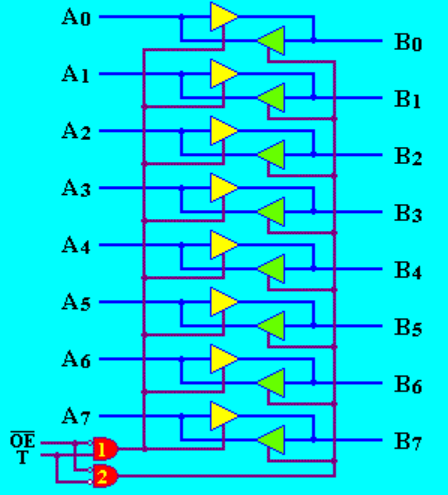
\includegraphics[scale=1]{part_8086CPU/part_8086CPU_pic/8286数据收发器.png}
    \caption{8286数据收发器}
\end{figure}
由8组首尾相连的反相器组成。$\overline{OE}=1$时禁止收发数据,输出低电平;$\overline{OE}=0$时允许收发数据,若T=1,传送方向为A到B(发送),反之为接收。

\noindentbf{8284时钟产生器}
\begin{figure}[H]
    \centering
    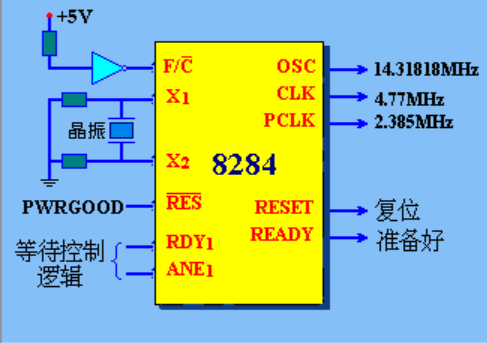
\includegraphics[scale=1]{part_8086CPU/part_8086CPU_pic/8284时钟发生器.png}
    \caption{8284时钟发生器}
\end{figure}
\begin{enumerate}
    \item $F/\overline{C}=0$时,输入频率由晶振决定,可以输出三种脉冲信号
    \item $\overline{RES}$接PWRGOOD,系统加电,四种直流输出电压($\pm 5,\pm 12$)正常后,送出PWRGOOD,经8284同步,产生RESET送到CPU的RESET引脚引起复位
    \item RDY、AEN与外部等待逻辑电路相连,经8284同步后可以产生READY信号送给CPU,以产生等待周期$T_w$
\end{enumerate}
\subsubsection{8088最大模式}
地址是20位,但无$\overline{BHE}$信号,数据线只有8位,所以8286只用一片。地址/数据复用线为$AD_7-AD_0$
\subsubsection{8088最小模式}
也要3片8282,在小系统中可以不用8286
\subsection{典型时序}
\subsubsection{读总线周期}
总线周期分为4个时钟周期,都是在时钟的下降沿触发。
\begin{figure}[H]
    \centering
    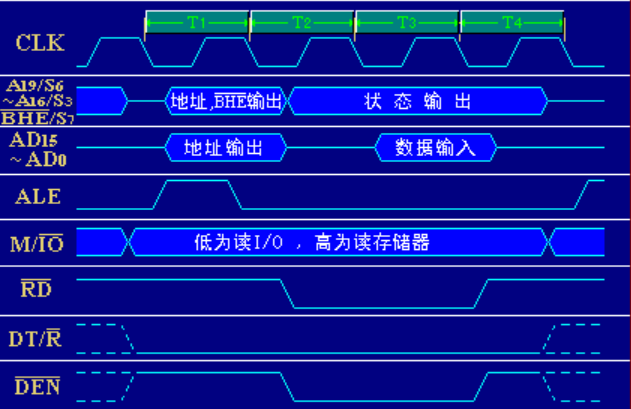
\includegraphics[scale=1]{part_8086CPU/part_8086CPU_pic/读总线周期.png}
    \caption{读总线周期}
\end{figure}
\subsubsection{写总线周期}
\begin{figure}[H]
    \centering
    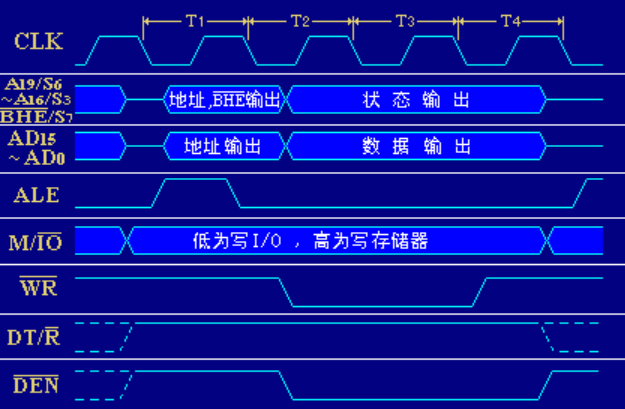
\includegraphics[scale=1]{part_8086CPU/part_8086CPU_pic/写总线周期.png}
    \caption{写总线周期}
\end{figure}
\subsection{存储器设计}
\subsection{SRAM 6264}
容量大小:8K×8

引脚及功能:
\begin{enumerate}
    \item $A_{12}-A_0$:13根地址线,选择芯片中$2^{13}$个存储单元中的任一个单元
    \item $I/O_7-I/O_0$:八根双向数据线,并行送数据
    \item $\overline{WE}$:写入允许信号
    \item $\overline{OE}$:读出允许信号
    \item $\overline{CE_1},\overline{CE_2}$:片选信号,两者均为低电平才能对芯片进行读写操作。其中一个作奇偶选择信号用。
\end{enumerate}
\subsection{SRAM 2114}
容量大小:1K×4

引脚及功能:
\begin{enumerate}
    \item $A_{9}-A_0$:13根地址线,选择芯片中$2^{13}$个存储单元中的任一个单元
    \item $I/O_4-I/O_0$:八根双向数据线,并行送数据
    \item $\overline{WE}$:写入允许信号
    \item $\overline{CS}$:片选信号
\end{enumerate}
\subsection{EPROM 2764}
EPROM允许用户将写入的内容用专门的擦除器擦除,允许反复擦除与重写。但是2764在正常使用时只能读出。
容量大小:8K×8

引脚及功能:
\begin{enumerate}
    \item $A_{12}-A_0$:13根地址线,选择芯片中$2^{13}$个存储单元中的任一个单元
    \item $O_7-O_0$:八根双向数据线,并行送数据
    \item $\overline{OE}$:读出允许信号
    \item $\overline{CE}$:片选信号
    \item PGM:编程脉冲控制
    \item $V_{pp}$:编程电压输入
    \item $V_{cc}$:工作电压,接+5V
\end{enumerate}
*编程方式时的引脚状态
\begin{enumerate}
    \item $A_{12}-A_0$:选中存储单元,逐字编程
    \item $\overline{OE}$:接+5V
    \item $\overline{CE}$:接+5V
    \item PGM:对每个单元编程时,从该引脚上输出一个50ms宽的正脉冲
    \item $V_{pp}$:接+21V到+25V
    \item $V_{cc}$:工作电压,接+5V
\end{enumerate}
\subsection{存储器系统连线图}
\begin{figure}[H]
    \centering
    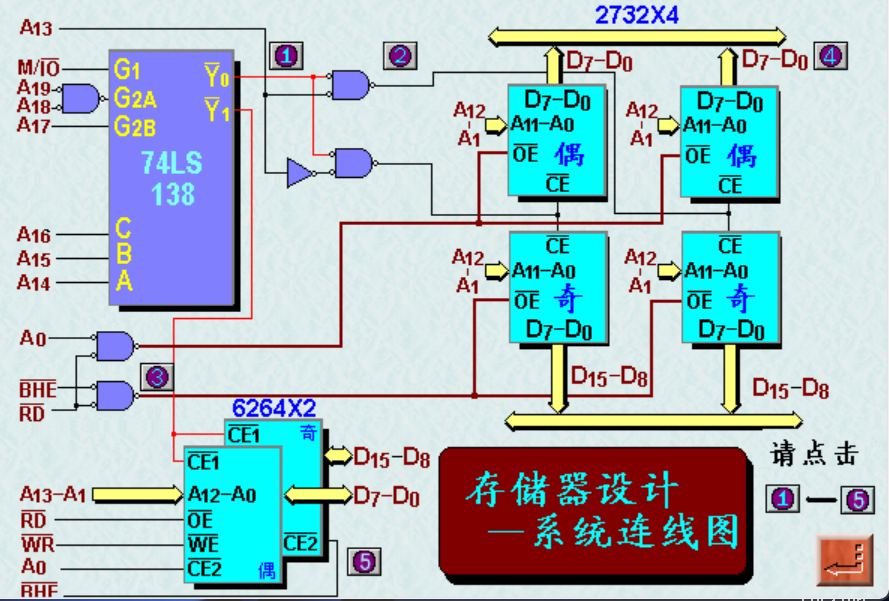
\includegraphics[scale=1]{part_8086CPU/part_8086CPU_pic/存储器系统连线图.png}
    \caption{存储器系统连线图}
\end{figure}

\chapter{指令系统}
\section{寻址方式}
\subsection{立即寻址}
操作数包含在指令中,它是一个8或16位常数,称为立即数。

示例
\begin{lstlisting}
    MOV AX,1860H
\end{lstlisting}
表示将1860H送入AX寄存器中。其中,立即数在代码段中,紧跟在操作码之后。
\subsection{寄存器寻址}
操作数包含在寄存器中,由指令指定寄存器名
\begin{lstlisting}
    MOV AX,BX
    MOV CH,AL
\end{lstlisting}
表示将寄存器BX中的数送入AX寄存器中。第二条指令说明低位和高位可以互相传数字
\subsection{存储器寻址}
操作数在存储器中。这种方式速度慢,表达方式最多,情况最复杂,要求能在1MB存储空间中寻址。段内偏移量也称有效地址EA。
\subsubsection{物理地址计算方法}
该类所有指令如图\ref{存储器物理地址计算图示}
\begin{figure}[H]\label{存储器物理地址计算图示}
    \centering 
    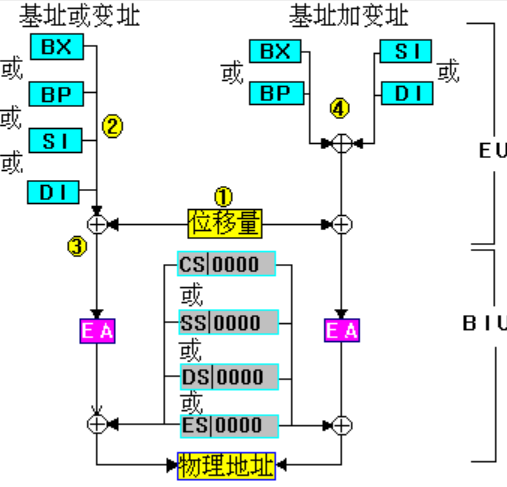
\includegraphics[scale=1]{part_指令系统/part_指令系统_pic/存储器物理地址计算图示.png}
    \caption{存储器物理地址计算图示}
\end{figure}
段寄存器可以是CS,SS,DS,ES;有效地址EA可以是
\begin{enumerate}
    \item 指令中直接指定的16位直接位移量,要加方括号
    \item BX/BP/SI/DI,{\color{red}{出现BP(不管是源处还是目的处)时默认使用SS提供段基址,但允许使用段超越前缀将SS修改为CS/DS/E,没有BP的,默认使用DS}}
    \item 位移量+基址/变址
    \item [BX/BP]+[SI/DI]+位移量,{\color{red}{画斜线的两者不能同时出现}}
\end{enumerate}
EA的24种表示法\ref{EA的24种表示方法}
\begin{figure}[H]
    \centering 
    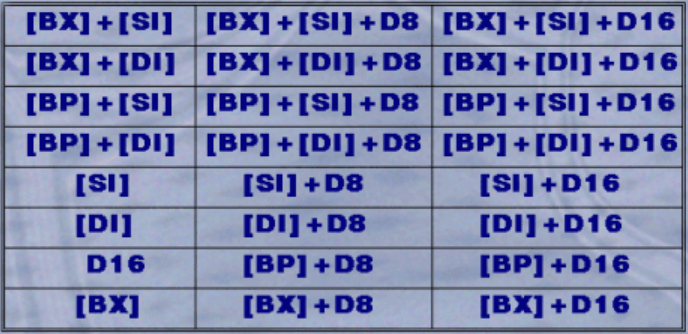
\includegraphics[scale=1]{part_指令系统/part_指令系统_pic/EA的24种表示方法.png}
    \caption{EA的24种表示方法}
    \label{EA的24种表示方法}
\end{figure}
\subsection{其他}
\subsubsection{隐含寻址}
指令中不明确指明操作数,但有隐含规定的 寻址方式。如:DAA对AL中的数进行十进制调整;CLI对中断标志清零
\subsubsection{一条指令包含几种寻址方式}
例如
\begin{lstlisting}
    MUL DL 
    ; AX<-AL*DL,源操作数为寄存器和隐含的寄存器AL
\end{lstlisting}
\subsubsection{IO端口寻址}
直接端口寻址:端口地址由指令直接给出,范围是00-FFH,若超出要先放到寄存器里。如
\begin{lstlisting}
    IN AL,40H
    OUT 83H,AL
\end{lstlisting}
间接端口寻址:端口地址由DX寄存器提供,其范围为0000-FFFFH
\begin{lstlisting}
    MOV DX,2F0H
    IN AL,DX ;;2F0H读入到AL
    MOV DX,300H
    OUT DX,AL ;;AL输出到300H
\end{lstlisting}
\subsubsection{转移类指令寻址}
详见控制转移指令
\section{数据传送}
\subsection{通用传送}
\subsubsection{MOV}
将操作数(字或字节)传送到目标操作数,源可为8位/16位通用寄存器(包括AX-DX,SI,DI,BP,SP),段寄存器(CS不能作为目的操作数),存储器或立即数。目的操作数不能为立即数,其他同源操作数。
四种数据来源的传送关系如图\ref{MOV指令的数据来源}
\begin{figure}[H]
    \centering 
    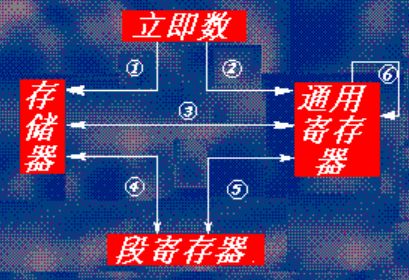
\includegraphics[scale=1]{part_指令系统/part_指令系统_pic/MOV指令的数据来源.png}
    \label{MOV指令的数据来源}
    \caption{MOV指令的数据来源}
\end{figure}
下面是一些示例
\begin{lstlisting}
    ; 立即数送存储器
    MOV [BX],0FFH
    ; 立即数送通用存储器
    MOV AL,30H
    MOV BL,'$'
    MOV AX,1250H
    MOV BX,OFFSET TABLE
    ; 存储器和通用寄存器相互传送
    MOV [BP],BX ; 带方框表示是段加偏移对应的存储器单元而不是BP本身的值受到改变
    MOV CL,5[BX]
    ; 存储器与段寄存器之间相互传送
    MOV [SI],DS
    ; 段寄存器和通用寄存器相互传送
    MOV ES,AX
    ; 通用寄存器之间相互传送
    MOV AX,DX
\end{lstlisting}
常见错误
\begin{lstlisting}
    ; 立即数不能作目的地
    MOV 60H,AL
    ; 存储器之间不能直接传送
    MOV [BX],[SI]
    ; CS不能作目的操作数
    MOV CS,AX
    ; 通用寄存器无IP寄存器
    MOV BX,IP
    ; 段寄存器之间不能直接传送
    MOV DS,ES 
    ; 数的长度不一致
    MOV CX,AL
\end{lstlisting}
\subsubsection{PUSH}
将源操作数入栈并使SP减二.{\color{red}低位先入栈}
\begin{lstlisting}
    PUSH AX ; 把AX入栈
\end{lstlisting}
\subsubsection{POP}
将当前SP指向的栈顶的一个字送到目的操作数中,并使SP+2.操作数可以是16位通用寄存器,DS/SS/ES或存储单元。{\color{red}堆栈操作总是以字为单位}
\begin{lstlisting}
    POP AX ; 先出栈的一个字节给到低位
\end{lstlisting}
\subsubsection{XCHG}
把字或字节的源操作数和目的操作数交换。可以发生在寄存之间或寄存器与存储器之间,但是段寄存器不能作操作数。
\begin{lstlisting}
    ; Right
    XCHG AX,BX
    XCHG [BI],CL 
    ; Wrong
    XCHG AX,0AF4H ;立即数不能交换
    XCHG SS,[SI] ; 段寄存器不参与交换
    XCHG [SI],[BX+1] ; 存储器之间不能直接交换
\end{lstlisting}
\subsubsection{XLAT}
将一个字节从一种代码转换成另一种代码。注意:
\begin{enumerate}
    \item 使用指令前必须先创建一个表格,将转换表的起始地址装入BX中
    \item AL存表头地址到所查找的某一项之间的位移量,根据位移量从表中查到转换后的代码值送入AL
    \item 表中最多存256字节
\end{enumerate}
典型的例子是用该指令将十进制数转换成七段显示管的代码
\begin{lstlisting}
    TABLE: DB 40H,79H,24H,30H,19H
           DB 12H,02H,78H,00H,18H ; 做表
           ... 
        LEA BX,TABLE ; 把表头地址给BX
        MOV AL,5 ; 把表内的偏移量给AL
        XLAT ; 此时AL中有‘5’的七段代码12H(表内从零开始数)
\end{lstlisting}
\subsection{输入输出}
\subsubsection{IN(OUT同理)}
把指定端口的内容读到AL(for byte)或AX(for word)中
\begin{lstlisting}
    ; 格式1:立即数指示端口
    IN AL,nn ;nn指代的8位端口的内容读到AL,nn=00-FFH
    IN AX,mm ;mm指代的16位端口读到AL,mm+1指代的16位端口读到AH.mm=00-FEH
    ; 格式2:用寄存器给端口号
    IN AL,DX ; DX=0000-FFFFH
    IN AX,DX ; DX=0000-FFFEH DX指代的16位端口读到AL,DX+1指代的16位端口读到AH
\end{lstlisting}
{\color{red}{当口地址大于FFH时,必须用格式2}}。典型示例:扬声器发声。
\subsection{地址目标}
这是一类专门用来传送地址码的指令
\subsubsection{LEA}
取源操作数地址的偏移量,传送到目的操作数所在的单元(load effective address)。{\color{red}源操作数必须是存储单元,目的操作数必须是除段寄存器以外的16位寄存器}
\begin{lstlisting}
    ; 注意区分LEA(取偏移地址)和MOV(取内容)
    ; 设SI=1000,DS=2000,(21000H)=1234,则
    LEA BX,[SI] ; BX=1000
    MOV BX,[SI] ; BX=1234
    ; 下面两段代码等效
    LEA BX,TABLE
    MOV BX,OFFSET TABLE
\end{lstlisting}
\subsubsection{LDS}
load DS:从源操作数指定的存储单元中取出4个字节的地址指针送进一对目的寄存器中(常用SI寄存器,但是不能是段寄存器)
load ES:与LDS基本相同但是后两个字节给到ES而非DS,目的操作数也常为DI而非SI
\begin{lstlisting}
    ; 设DS=0100,BX=0020,(01020H)=26A0H,(01022H)=B500H
    LDS SI,[BX] ; 低位两个字节给SI,SI=26A0,高位两字节给DS,DS=B500
    LES DI,[BX] ; DI=26A0,ES=B500
\end{lstlisting}
\subsection{标志传送}
\subsubsection{LAHF}
load AH flags:将SF,ZF,AF,PF,CF送到AH的7,6,4,2,0位,而5,3,1位为任意值。
\subsubsection{SAHF}
send AH flags:将AH的7,6,4,2,0位送到SF,ZF,AF,PF,CF,而高位flag(OF,DF,IF,TF)不受影响。
\subsubsection{PUSHF/POPF}
将整个标志寄存器的内容压栈/出栈,并使SP-2/+2(仍然是低位先入栈,高位先出栈)
\section{算数运算}
该类所有指令如图\ref{算数运算指令}
\begin{figure}[H]
    \centering 
    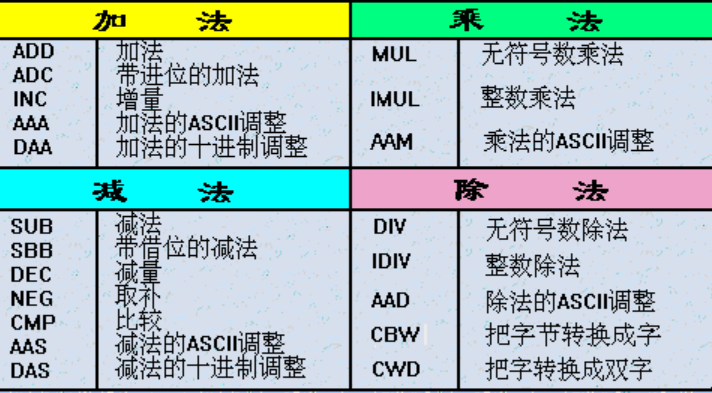
\includegraphics[scale=1]{part_指令系统/part_指令系统_pic/算数运算指令.png}
    \label{算数运算指令}
    \caption{算数运算指令}
\end{figure}
\subsection{加法}
\subsubsection{ADD}
目的数被赋值为“目的数+源”
\begin{lstlisting}
    ; RIGHT
    ADD AL,45H
    ADD BL,DL 
    ADD [BX],CL
    ; Wrong
    ADD 85H,AL ; 立即数不能被赋值
    ADD 5[BX],[BP] ; 两个存储器内容不能直接相加
    ADD BX,CL ; 字节和字不能相加
\end{lstlisting}
加法指令结束后将影响六个标志位,如何解释这些标志位(是无符号数相加还是有符号数相加决定是进位还是溢出)取决于程序员。
\subsubsection{ADC}
add carry:带进位的加法指令。目的=目的+源+CF
\subsubsection{INC}
increment:增量指令,对目的操作数加1.操作后影响AF,OF,PF,SF,ZF,但不影响CF
\begin{lstlisting}
    INC BL 
    INC BYTE PTR[BX] ; 对内存字节单元内容+1
    INC WORD PTR[BX] ; 对内存字单元内容+1
\end{lstlisting}
\subsubsection{AAA}
ascii-adjusted add:加法的ASCII调整指令。用ADD或ADC对两个非压缩十进制数或ASCII表示的十进制数作加法,且运算结果保留在AL中后,用AAA可以将运算结果调整为一位非压缩十进制数,仍然放在AL中。若AF=1,则表示高位有进位,进到AH中。

*非压缩十进数(BCD数):高四位全为零
例题图\ref{AAA指令例题}
\begin{figure}[H]
    \centering 
    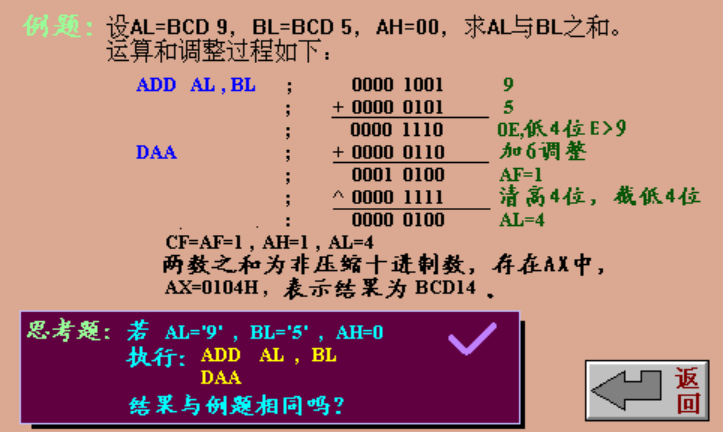
\includegraphics[scale=1]{part_指令系统/part_指令系统_pic/AAA指令例题.png}
    \label{AAA指令例题}
    \caption{AAA指令例题}
\end{figure}
\subsubsection{DAA}
decimal-adjusted add:加法的十进制调整指令。将两个压缩的BCD数相加的结果调整为正确的压缩BCD数,相加结果必须在AL中才能使用DAA。
例题图\ref{DAA指令例题}
\begin{figure}[H]
    \centering 
    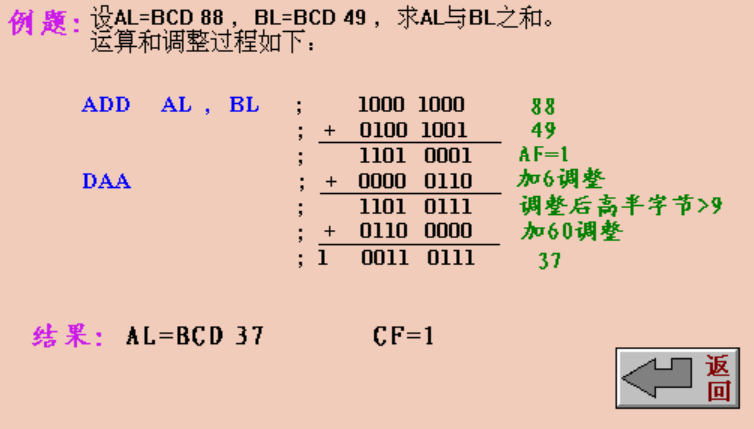
\includegraphics[scale=1]{part_指令系统/part_指令系统_pic/DAA指令例题.png}
    \label{DAA指令例题}
    \caption{DAA指令例题}
\end{figure}
\subsection{减法}
\subsubsection{SUB}
将目的操作数减去源操作数,结果送回目的操作数
\begin{lstlisting}
    SUB AL,BL ; 将AL-BL的值送到AL
\end{lstlisting}
\subsubsection{SBB}
带借位的减法:两个操作数相减后还要减去进位/借位标志CF的值,返回到目的操作数
\begin{lstlisting}
    SUB AL,CL ; 将AL-CL-CF的值送到AL
\end{lstlisting}
\subsubsection{DEC/NEG}
decrease:减量指令,对目的操作数减1,结果送回目的操作数。
\begin{lstlisting}
    DEC BX ; BX-1的值返回到BX
    DEC WORD PTR[BP] ; 堆栈段中位于[BP]偏移量处的字减1
\end{lstlisting}
negative:取反指令,即用0减去操作数再送回
\begin{lstlisting}
    MOV AL,00000101B ; AL=5
    NEG AL ;AL=11111011B (-5的补码)
\end{lstlisting}
\subsubsection{CMP}
compare:将目的数减去源操作数,结果不返回,但是反映在标志位上。这种指令用于希望在不破坏原数的情况下比较大小
\subsubsection{AAS/DAS}
ascii-adjusted sub:减法的ASCII调整。在减法指令后对两个非压缩的十进制数或ASCII码表示的十进制数相减后,在AL中得到的结果进行调整,使AL中得到正确的非压缩十进制数之差,若有借位,则CF置一。

低四位大于9/或AF=1时,用减6(而非+6)调整。

DAS类似,但是当当高4位大于9时,要减60H调整。
\subsection{乘法}
\subsubsection{MUL}
把源操作数和累加器中的数都当成无符号数。源操作数可以是字节或字
\begin{lstlisting}
    MUL DL ; DL*AL的结果放到AH(高)和AL(低)中
    MUL DX ; DX*AX的结果放到DX(高)和AX(低)中
\end{lstlisting}
\subsubsection{IMUL}
integer mul:整数乘法指令。把源和累加器中的数都当作有符号数相乘。若执行IMUL指令后,乘积的高半部分不是低半部分的符号扩展,则表示高位为有效位,是积的一部分,于是置CF=1,OF=1.若高半部分全是0或1,表明仅包含了符号位,CF=0,OF=0。
\subsubsection{AAM}
ascii-adjusted mul:乘法的ascii调整。对已经存放在AL中的两个非压缩的十进制数相乘的结果进行十进制数的调整,使得在AX中得到正确的非压缩十进制数的乘积。高位放在AH,低位放在AL。
\subsection{除法}
\subsubsection{DIV}
\begin{lstlisting}
    DIV BL ; AX/BL,商放在AL,余数放在AH
    DIV BX ; 若源操作数是字,则32位被除数放在DX(高)和AX中,相除后商放在AX,余数放在DX
\end{lstlisting}
如果被除数只有8位,则必须将其放在AL中,并把AH清零。如果被除数只有16位,则必须将其放在AX中,并把DX清零。{\color{red}{DIV执行后,所有标志无定义}}
\subsubsection{IDIV}
整数除法(带符号位除法):操作数、商和余数全是带符号数,并且规定余数的符号与被除数相同。所有标志位无定义。

{\color{red}{若被除数的高位绝对值大于除数的绝对值,也即商数超过了目标寄存器所能存放的数的范围,则计算机会出现除法错中断,商和余数不确定}}
\subsubsection{CBW}
把寄存器AL中的符号位扩充到AH的所有位,这是AH称为AL的符号扩充。即若AL的$D_7=0$,则AH的所有位都置零。反之都置一。
\subsubsection{CWD}
把AX的符号位扩充到DX中。
\subsubsection{AAD}
除法的ASCII调整:在做除法之前,把(AX中的)BCD码转化位二进制数。即执行AAD后,AL=AH*10+AL,AH=00H
\section{逻辑移位}
该类所有指令如图\ref{逻辑运算与移位指令}
\begin{figure}[H]
    \centering 
    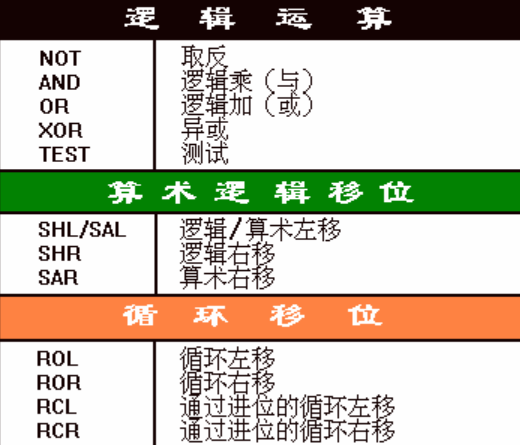
\includegraphics[scale=1]{part_指令系统/part_指令系统_pic/逻辑运算与移位指令.png}
    \label{逻辑运算与移位指令}
    \caption{逻辑运算与移位指令}
\end{figure}
\subsection{逻辑运算}
\subsubsection{NOT}
按位取反,返回到原位置
\subsubsection{AND,OR,XOR}
按位与/或/异或,结果返回到目的操作数
\subsubsection{TEST}
对两个操作数逻辑与,并修改标志位但不送回结果,操作后两个操作数都不变。往往后接转移指令。
\subsection{算数移位}
一般格式:“指令 目的,计数值”。计数次数=1时可以直接给出,否则要先把计数值送到CL
\subsubsection{SAL/SHL}
shift (arithmetic) left:将寄存器或存储器中的目的操作数各位左移,每移位一次,最低有效位LSB补零,最高有效位MSB进入CF。SHL与SAL一样。
\subsubsection{SHR}
shift right:将寄存器或存储器中的目的操作数各位右移,每移位一次,最低有效位LSB进入CF,最高有效位MSB补零。SHL与SAL一样。
\subsubsection{SAR}
与SHR类似。只是最高位不是补零而是保持不变。每移位一次相当于带符号数除以2.
\subsection{循环移位}
\subsubsection{ROL}
rotate left:循环左移。最高位不止给CF,还给到最低位
\subsubsection{ROR}
rotate right:循环右移。最低位不止给CF,还给到最高位
\subsubsection{RCL}
rotate carry left:通过进位位循环左移。把进位位放在最高位的左边一起参与左移。RCR也是是把进位位放在最高位的左边,一起参与右移。
\section{字符串}
字符串操作指令共有5条,每条指令有3种格式,指令后加B是字节操作,加W是字操作。

字符串指令隐含约定:
\begin{enumerate}
    \item 源串起始地址位DS:SI,允许用段超越前缀修改段地址DS
    \item 目的串起始地址为ES:DI,禁止使用段超越前缀修改ES
    \item 每次执行一次字符串指令,指针SI和DI自动修改
    \item DF标志位控制字符串处理方向。CLD使DF为0,为递增方向;STD使DF为1,递减。字节串每次SI,DI变1,字串每次变2
    \item 要处理的字符串长度放在CX寄存器中。可以在基本字符串指令前加重复前缀,加快串运算指令的执行速度。
\end{enumerate}
\subsection{传送}
\subsubsection{MOVS}
mov string
\begin{lstlisting}
    MOV CX,4 ;即要传送的字节数为4
    CLD ; 使DF=0,自增方向
    REP MOVSB ; 将DS:SI中的四个字节送到ES:DI中
\end{lstlisting}
\subsubsection{重复前缀}
\begin{enumerate}
    \item REP 常与MOVS或STOS连用
    \item REPE/REPZ 相等/结果为零则重复,常与CMPS连用,重复比较串数据知道两个字符不相等或CX=0
    \item REPNE/REPNZ 不相等/结果非零则重复。常与SCAS连用,重复查找某个数据知道ZF=1(找到了)或CX=0
\end{enumerate}
\subsection{比较}
\subsubsection{CMPS/CMPSB/CMPSW}
将源串内容减去目的串,并自动修改SI、DI,比较结果反映在FLAGS上,用来比较两个字符串是否相等。常用于密码验证
\begin{lstlisting}
    MOV CX,4
    CLD
    REPZ CMPS ; 将DS:SI指向的源串减去ES:DI指向的 目的串,若两串当此比较结果相同,ZF=1且CX不为零,则继续比较
\end{lstlisting}
\subsection{扫描}
\subsubsection{SCAS}
scan string:字符串扫描指令,从AL或AX寄存器的内容减去附加段中以DI为指针的目的元素,结果反映在标志位上,但是不改变操作数。被搜索的字(节)称为关键字
\begin{lstlisting}
    MOV DI,OFFSET STRING ;字串偏移地址
    MOV CX,COUNT ; 字符串长度即为最大重复次数
    MOV AL,'A' ; 关键字送入AL
    CLD
    REPNE SCASB 
    JZ FIND ; 搜索到,转出
    MOV DI,0 ; 没找到,DI=0
    FIND:
    MOV BX,DI ; BX=搜索次数
    HLT ; 停机
\end{lstlisting}
\subsection{装入}
\subsubsection{LODS}
load string:字符串装入指令。将DS:SI指向的源串送到AX(对字)或AL(对字节)中,并修改SI,加重复前缀无意义,因为累加器只能存储一个数据,重复操作后也只保留最后写入的数据。
\subsection{存储}
\subsubsection{STOS}
store string:数据串存储指令,与LODS相对。将累加器AL或AX中的一个字节或字传送到附加段中以DI为目标指针的目的串中,同时修改DI,以指向串中的下一个单元。与REP连用,常用于重复使用累加器中的一个常数,将串初始化(比如置为全0)
\begin{lstlisting}
    ; 设DI=2000H 
    MOV AX,0000H 
    CLD 
    STOSW ; 这一步执行完后,DI=2002H
    MOV AX,00FFH
    MOV CX,100H
    REP LODSW ???!!!; 这一步执行完后,DI=2202H,从ES:2002到ES:2201,全部装入00FFH
\end{lstlisting}
\section{控制转移}
该类所有指令如图\ref{控制转移指令}
\begin{figure}[H]
    \centering 
    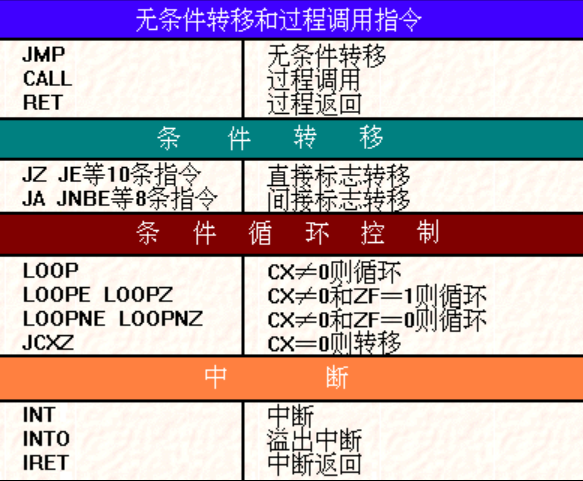
\includegraphics[scale=1]{part_指令系统/part_指令系统_pic/控制转移指令.png}
    \label{控制转移指令}
    \caption{控制转移指令}
\end{figure}
\subsection{无条件转移}
\begin{table}
    \centering
    \begin{tabular}{ccc}
        \hline 
        类型 & 方式 & 寻址目标  \\ \hline
        段内转移 & 直接 & 立即短转移(8位) \\ \hline
        段内转移 &直接& 直接近转移(16位)\\ \hline
        段内转移 & 间接 &寄存器(16位) \\ \hline
        段内转移 & 间接 &存储器(16位)\\ \hline
        段间转移 & 直接 & 立即转移(32位) \\ \hline
        段间转移 & 间接 & 存储器(32位)\\ \hline
    \end{tabular}
\end{table}
\subsubsection{段内直接转移指令}
\noindentbf{JMP SHORT PROGS}
段内短转移指令:指令执行后,跳转到标号为PROGS处执行。PROGS的偏移地址和JMP指令后下条地址之间的范围在-128-+127之间
\noindentbf{JMP (NEAR PTR) PROG}
PROG的偏移地址和JMP指令后下条地址之间的范围在-32768-+32767之间,若超出这个范围,汇编语言自动用向回转移的方法解决。该指令可以使程序转移到段内任何位置执行。
\subsubsection{段内间接转移指令}
有效地址可以是寄存器也可以是存储器单元
\begin{lstlisting}
    JMP BX ; 假设BX=4500H,则指令执行后将IP赋值为4500H
\end{lstlisting}
\subsubsection{段间直接转移指令}
\begin{lstlisting}
    JMP FAR PTR PROG ; 执行后,PROG所在的段内偏移量给IP,段地址给CS,即程序转到PROG处执行
\end{lstlisting}
\subsubsection{段间间接转移指令}
\begin{lstlisting}
    JMP DWORD PTR [SI+0125H]
\end{lstlisting}
当程序执行到上述指令时,从DS:SI+0125H这一数据段单元中取出两个字,低位给到IP,高位给CS,从而转到新的代码段执行。
\subsection{过程调用}
程序将某些独立的程序段模块化,称为过程或子程序。用CALL能调用这些过程。过程执行完后通过RET返回主程序,RET可以带参数。

子程序以PROC开头,以EDNP结束,RET位于ENDP之前
\subsubsection{段内直接调用}
\begin{lstlisting}
    MAIN PROC FAR 
    ... 
    CALL SUBPRO ;调用子程序,CALL指令的后一条指令的IP入栈,转入子程序执行。
    ... 
    RET 
    SUBPRO PROC NEAR ;子程序,NEAR说明是近过程
    ... 
    RET  ; 返址出栈,CALL指令的下一条指令执行
    SUBPRO ENDP 
    MAIN ENDP ; MAIN看作是DOS调用的一个子过程,其属性必须为FAR
\end{lstlisting}
\subsubsection{段间直接调用}
\begin{lstlisting}
    SEGM SEGMENT ;程序段A
    ... 
    CALL SUMPRO ; 段内调用子过程
    SUBPRO PROC FAR ; 进入远过程,并用FAR说明 
    ... 
    RET ; 远返回,从栈中弹出双字CS:IP 
    SUBPRO ENDP ; 返回CALL的下一条指令执行
    ... 
    SEGM ENDS 
    SEGB SEGMENT ; 程序段B
    ... 
    CALL SUBPRO ; 调用程序段A中的远过程,CALL的下一条指令的CS:IP入栈,转入SUBPRO执行
    ... 
    ENDS 
    SEGB ENDS 
\end{lstlisting}
与JMP的对比
\begin{enumerate}
    \item CALL无短调用指令
    \item JMP指令执行后不再返回原程序
    \item CALL指令的RET带参数n表示从栈中弹出返址后,再从栈中弹出n(0000-FFFFH)个字节的数据
\end{enumerate}
\subsection{条件转移}
根据上一条指令执行后CPU设置的状态标志做测试条件决定是否转移,满足条件才转移。所有的条件转移指令均为短转,目的地址都用标号表示
\subsubsection{直接标志转移指令}
\begin{table}[H]
    \centering 
    \begin{tabular}{ccc}
        \hline 
        指令助记符 & 测试条件 & 指令功能 \\ \hline
        JC   &      CF=1& 有进位 \\
        JNC    & CF=0 &无进位\\
        JZ/JE& ZF=1 &结果为0/相等\\
        JNZ/JNE &ZF=0 &不为零/不相等\\
        JS& SF=1 &符号为正\\
        JNS& SF=0 &符号为负\\
        JO &OF=1& 溢出\\
        JNO& OF=0 &无溢出\\
        JP/JPE& PF=1 &奇偶位为1/为偶\\
        JNP/JPO& PF=0 &奇偶位为0/为奇\\ \hline
    \end{tabular}
\end{table}
\begin{lstlisting}
    ADD AL,BL
    JC NEXT ;此处若CF=1,则转到NEXT处执行
    ... 
    NEXT:MOV AL,BL
\end{lstlisting}
\subsubsection{间接标志转移指令}
不是简单的通过标志状态位来决定是否跳转。而是经过一定的逻辑运算(更贴近数学逻辑)
\begin{table}[H]
    \centering 
    \begin{tabular}{ccc}
        \hline 
        类别 & 指令助记符 & 指令功能 \\ \hline
        无符号数比较 & JA/JNBE & 高于/不低于等于\\
        无符号数比较 & JAE/JNB&高于等于/不低于\\
        无符号数比较 & JB/JNAE&低于/不高于等于\\
        无符号数比较 & JBE/JNA&低于等于/不高于\\
        带符号数比较 & JG/JNLE&大于/不小于等于\\
        带符号数比较 & JGE/JNL&大于等于/不小于\\
        带符号数比较 & JL/JNGE&小于/不大于等于\\
        带符号数比较 & JLE/JNG&小于等于/不大于\\ \hline
    \end{tabular}
\end{table}
带符号数比较时,负数视为小于正数。
\subsection{条件循环控制}
增强型的条件转移指令,用于控制一个程序段的重复执行,重复次数在CX中
\subsubsection{LOOP}
后加短标号,循环标号指定程序CX次
\begin{lstlisting}
    MOV CX,8
    MOV BX,00 
    NEXT:MOV AL,[BX];加法程序 
    ADD AL,5
    MOV [BX],AL 
    INC BX 
    LOOP NEXT ;一共做8次加法
\end{lstlisting}
\subsubsection{LOOPE/LOOPZ}
相等或结果为零则循环指令
\subsubsection{LOOPNE/LOOPNZ}
不相等结果不为0则循环指令
\subsubsection{JCXZ}
若CX=0则跳转指令,主要用在循环程序开始处,为了使程序跳过循环,只要事先把CX清零即可
\subsection{中断指令}
\subsubsection{INT n}
软中断指令,将标志寄存器FLAGS内容入栈。断点(INT n的下条指令)基址:偏移地址入栈。从n*4开始的单元中取出中断服务程序入口地址的CS:IP转相应程序执行
\subsubsection{IRET}
中断返回指令,总是被安排在中断服务程序的出口处。功能是:
\begin{enumerate}
    \item 从栈中弹出断点送到CS和IP中
    \item 弹出FLAGS内容
    \item 按CS:IP的值返回断点,执行原来的程序
\end{enumerate}
\subsubsection{INTO}
溢出中断指令。当溢出标志OF=1,再执行INTO时,自动产生类型号为4的中断指令。即执行INT 4指令 

主要用于带符号数加减运算产生溢出错时的处理
\begin{lstlisting}
    ADD AL,BL 
    INTO ;如OF=1,则产生INT 4中断。此处若不安排INTO,溢出也不会产生中断,可能引发未知后果
\end{lstlisting}
\section{控制指令}
该类所有指令如图\ref{控制指令}
\begin{figure}[H]
    \centering 
    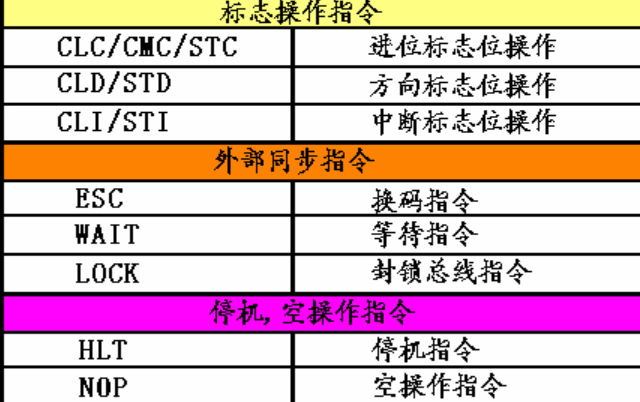
\includegraphics[scale=1]{part_指令系统/part_指令系统_pic/控制指令.png}
    \label{控制指令}
    \caption{控制指令}
\end{figure}
\subsection{标志操作指令}
这类指令可以直接对一些标志位进行操作。
\begin{table}[H]
    \centering 
    \begin{tabular}{cc}
        \hline 
        指令助记符 & 作用 \\ \hline 
        CLC &CF=0\\
        CMC &CF=$\overline{CF}$\\
        STC &CF=1\\
        CLD &DF=0(增量)\\
        STD &DF=1(减量)\\
        CLI &IF=0(不响应可屏蔽中断)\\
        STI &IF=1(响应可屏蔽中断)\\ \hline 
    \end{tabular}
\end{table}
\subsection{外部同步指令}
\subsubsection{ESC}
换码指令:协处理器8087和8086系统总线互联。一旦取出一条ESC指令,8087的BUSY引脚信号变高,通过它使8086的$\overline{TEST}$变高,协处理开始工作。完毕后向8086的$\overline{TEST}$发出低电平,执行后续指令。
\subsubsection{WAIT}
等待指令。通常跟在ESC之后。CPU执行ESC后,CPU处于等待状态,期间不断检测$\overline{TEST}$引脚,若为高,则重复执行WAIT。
\subsubsection{LOCK}
封锁总线指令。这是一种前缀,可加在任何指令的前端使8086的总线封锁信号有效。带有LOCK前缀的指令在执行过程中将禁止其他处理器使用总线
\begin{lstlisting}
    LOCK MOV AX,05H ;封锁总线指令
\end{lstlisting}
\subsection{停机和空操作}
\subsubsection{HLT}
停机指令。使CPU进入暂停状态,不进行任何操作。当下列情况之一发生时脱离暂停状态。常用HLT指令等待中断的出现
\begin{enumerate}
    \item 在RESET线上加复位信号
    \item NMI引脚上有中断请求信号
    \item 当IF=1,INTR引脚上出现中断请求信号时
\end{enumerate}
\subsubsection{NOP}
空操作或无操作指令。不完成任何操作。通常被插在其他指令之间,在循环等操作中增加延时
\end{document}
